\section{The Limit of a Sequence}
    \textbf{Definition 2.2.1.} A \textit{sequence} is a function whose domain is \textbf{N}.
    \newline Each of the following are common ways to describe a sequence.
    \begin{enumerate}
        \item $(1, \frac{1}{2}, \frac{1}{3}, \dots)$
        \item $(\frac{1}{n})_{n=1}^\infty$
        \item $(a_n)$, where $a_n = 1/n$ for each $n \in \textbf{N}$
        \item $(x_n)$, where $x_1 = 2$ and $x_{n+1} = \frac{x_n + 1}{2}$
    \end{enumerate}
    We do not need to start the sequence at $n=1$, we can start it at $n=0$ or $n=n_0$ where $n_0 \in \textbf{N}$.
    \newline
    \textbf{Definition 2.2.3 (Convergence of a Sequence).} A sequence $(a_n)$ \textit{converges} to a real number $a$ if, for every positive number $\epsilon$, there exists an $N \in \textbf{N}$ such that whenever $n \geq N$ it follows that $|a_n - a| < \epsilon$.
    \newline \indent To indicate that $(a_n)$ converges to $a$, we write either $\lim_{n \rightarrow \infty} a_n = \lim a_n = a$ or $(a_n) \rightarrow a$.
    \newline
    \textbf{Definition 2.24.} Given a real number $a \in \textbf{R}$ and a positive number $\epsilon > 0$, the set $$V_{\epsilon}(a) = {x \in \textbf{R}: |x - a| < \epsilon}$$ is called the $\epsilon$-\textit{neighborhood of a}.
    \begin{center}
        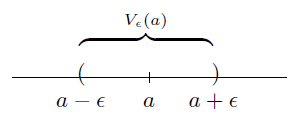
\includegraphics[width=150pt]{epsilon-neighborhood.png}
    \end{center}
    \textbf{Definition 2.2.3B (Convergence of a Sequence: Topological Version).} A sequence $(a_n)$ converges to $a$ if, given any $\epsilon$-neighborhood $V_{\epsilon}(a)$ of $a$, there exists a point in the sequence after which all of the terms are in $V_{\epsilon}(a)$. In other words, every $\epsilon$-neighborhood contains all but a finite number of the terms of $(a_n)$.
    \begin{center}
        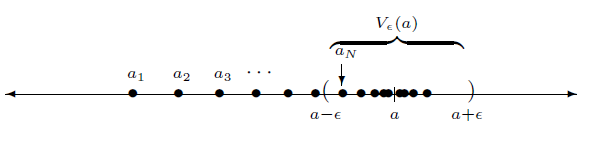
\includegraphics[width=200pt]{convergence.png}
    \end{center}
    \subsection*{Quantifiers}
        \begin{center}
            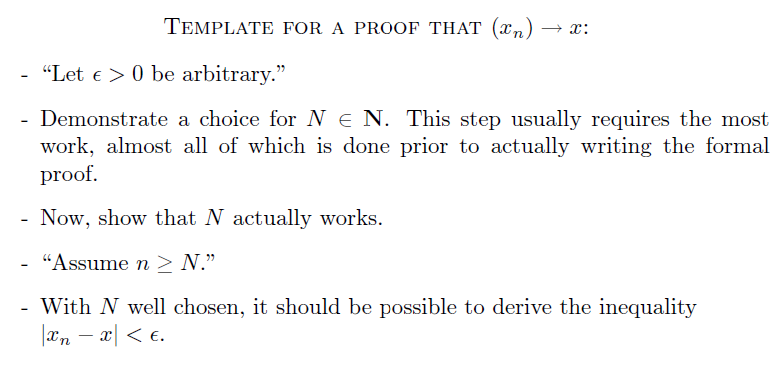
\includegraphics[width=300pt]{template.png}
        \end{center}
    \subsection*{Divergence}
        \textbf{Definition 2.2.8.} A sequence that does not converge is said to \textit{diverge}.
        